\section{System Modelling}\label{sec:modelling}

\subsection{System Model}

\subsubsection{Differential equation describing the motion of the mass}

The brief describes the suspension as a mass $m$ carrying a spring of stiffness $k$ and a
viscous damper of coefficient $b$, driven by an applied force $F(t)$ proportional to the
input voltage. Summing forces on the mass, with $x(t)$ the displacement of the mass from
its rest position,

\begin{equation}\label{eqn:eom}
    m\ddot{x}(t) = -b\dot{x}(t) - kx(t) + F(t).
\end{equation}

The spring force opposes displacement and the damping force opposes velocity, which is
where both minus signs come from. Every parameter is scaled to the mass, so $m = 1$
throughout and $k$ and $b$ carry units of stiffness and damping per unit mass. The system
starts at rest, so all initial conditions are zero.

\subsubsection{Transfer function derived from the differential equation}

Taking the Laplace transform of Equation~\ref{eqn:eom} with zero initial conditions, and
writing $X(s) = \mathcal{L}\{x(t)\}$ and $F(s) = \mathcal{L}\{F(t)\}$,

\begin{equation}
    s^2X(s) + bsX(s) + kX(s) = F(s),
\end{equation}

so the transfer function from applied force to displacement is

\begin{equation}\label{eqn:tf}
    \frac{X(s)}{F(s)} = \frac{1}{s^2 + bs + k}.
\end{equation}

What the simulator applies, and what the log records, is an input $u(t)$ rather than a force.
The brief states only that the force is proportional to that input, so $F(t) = \alpha u(t)$
for a constant $\alpha$ that is not given and has to be identified along with $k$ and $b$.
The transfer function from the logged input to the measured displacement is therefore

\begin{equation}\label{eqn:tf_input}
    G(s) = \frac{X(s)}{U(s)} = \frac{\alpha}{s^2 + bs + k}.
\end{equation}

This is second order with no zeros, so its behaviour is fixed entirely by the three
constants. Comparing Equation~\ref{eqn:tf_input} against the canonical second order form on
the course formula sheet,

\begin{equation}\label{eqn:canonical}
    G(s) = \frac{A\omega_n^2}{s^2 + 2\zeta\omega_n s + \omega_n^2}
\end{equation}

gives the three identities the rest of the report rests on,

\begin{equation}\label{eqn:identities}
    \omega_n = \sqrt{k}, \qquad
    \zeta = \frac{b}{2\sqrt{k}}, \qquad
    A = G(0) = \frac{\alpha}{k}.
\end{equation}

Here $A$ is the steady state gain in metres per volt, $\omega_n$ the undamped natural
frequency in rad/s and $\zeta$ the dimensionless damping ratio. Equation~\ref{eqn:identities}
is what turns control quantities into physical ones. Measuring $A$, $\zeta$ and $\omega_n$
is the same as measuring $k$, $b$ and $\alpha$, since $k = \omega_n^2$, $b = 2\zeta\omega_n$
and $\alpha = Ak$.

Note that $A = 1/k$ only when $\alpha = 1$, that is, only if the input is the force itself in
the units Equation~\ref{eqn:eom} assumes. That is an assumption about the simulator, not a
result, so it is not made here. Section~\ref{sec:system_id} measures $A$ and $\omega_n$
independently and uses the two together to recover $\alpha$, which doubles as a check. An
$\alpha$ far from unity means the input column is scaled.

\subsection{Methodology}

The simulator is signed on with my student number so the plant keyed to it is loaded, then
\textbf{Laboratory Testing} is selected. \textbf{Start Step Test} is deliberately not used. It steps the height of the aircraft, not the suspension input, so it does not produce
the clean step the analysis needs. Logging writes
\texttt{F34BSuspensionTestData.csv} with time, input and output displacement columns at a
100~ms sample period. Figure~\ref{fig:bench} shows the panel and the test dialog carrying
the settings used for the step run.

\begin{enumerate}
    \item A step of size $1$~V is applied through \textbf{Offset Input} and
          logged until the response is visibly flat, so the final value is a genuine steady
          state and not a point on a still decaying curve.
    \item The steady state gain follows from $G(0)$ in Equation~\ref{eqn:canonical}, the
          damping ratio from the overshoot and the natural frequency from the damped period,
          as set out in Section~\ref{sec:step}.
    \item Sinusoids are then applied one at a time at the frequencies listed in
          Table~\ref{tab:freq}, each logged for long enough that the transient has died away
          before the part of the record that is used for fitting.
    \item Each log is processed by the script in Appendix~\ref{sec:appendix}, which fits
          amplitude and phase at the known drive frequency by least squares rather than
          reading peaks by eye, since 100~ms sampling is too coarse for peak picking to be
          reliable. Both columns of the log are fitted and the reported phase is the
          difference between them, so it is measured from the input as recorded rather than
          from the drive as commanded. That matters for Section~\ref{sec:validation}: a lag
          measured between two columns of the same file cannot be an artefact of when the
          log was started.
\end{enumerate}

\begin{figure}[htbp]
    \centering
    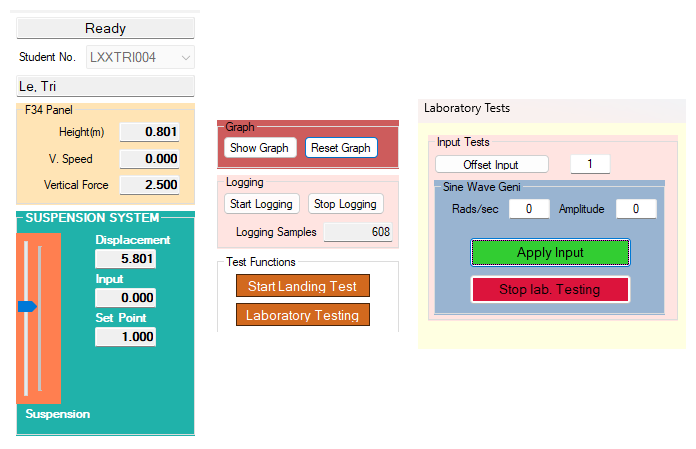
\includegraphics[width=0.92\textwidth]{figures/sim_bench.png}
    \caption{The simulator configured for the step test. The plant is keyed to the student
             number in the top field, so the left column both identifies which plant was
             loaded and reads the $5.801$~m the suspension settled at. On the right,
             \textbf{Offset Input} is $1$ with both sine fields at zero, which is how the
             $1$~V step is applied. The sinusoid runs use the same dialog with
             \textbf{Offset Input} returned to zero and the frequency and amplitude entered
             instead. \textbf{Start Logging} in the middle column opens the CSV and
             \textbf{Logging Samples} counts what has been written to it.}
    \label{fig:bench}
\end{figure}

Two sources of uncertainty need stating before any numbers appear. The logger writes
displacement to $0.001$~m, so any single reading is only known to $\pm 0.5$~mm, and that is the
limit on everything read off the step response. The 100~ms sample period is the other
candidate. A true peak falling between samples reads low and would bias $\zeta$ high. That
effect turns out to be small. Evaluating the identified model at the peak and half a sample
past it puts the worst case at $0.1$~mm, a tenth of a resolution step. The damped period is
$7.4$~s, so $100$~ms is $1.4$\% of it. Quantisation dominates and sampling does not, so the
resolution is the limitation this report carries forward.

One convention follows from the setup rather than from any uncertainty. The step is applied
on top of a non-zero resting displacement, so every amplitude quoted here is a change from
the pre-step baseline, not an absolute displacement.
